\subsection{Empfang von Daten}

Die Daten müssen auf beiden \ac{uC} ordnungsgemäß empfangen werden. Die Implementation unterscheidet sich hierbei stark. Der STM32 ermöglicht
die Nutzung seiner \ac{DMA}-Funktionalität, während auf dem ESP8266 eine Interruptbasierte Abfrage implementiert wird.

\subsubsection{STM32: Strukturvariable DMA\_STRUCT}

Aus Gründen der Übersichtlichkeit wurde für die Datenverarbeitung des STM32 eine Strukturvariable definiert, welche hiermit eingeführt wird.
Die Strukturvariable \lstinline!DMA_STRUCT! enthält mehrere weitere Variablen für Flags und Zähler.

\begin{lstlisting}
typedef struct
{
    volatile uint8_t  t_flag;   
    uint8_t tx_flag;			
    uint16_t timer;             
    uint16_t prevCOUNT;         
} DMA_STRUCT;
\end{lstlisting}

Die Flags \lstinline!t_flag! und \lstinline!tx_flag! dienen der Identifikation von Interrupts, welche durch im Falle von \lstinline!t_flag! durch ein
Timeout ausgelöst wurden oder im Falle von \lstinline!tx_flag! durch das erfolgreiche Senden von Daten. Die Variable \lstinline!timer! legt 
die Zeitkonstante für den Timeout fest, während \lstinline!prevCOUNT! einen Zähler speichert, der in \ref{subsub: Empfang} genauer erklärt wird.   

\subsubsection{STM32: Konfiguration des UART}
Wichtig bei der Konfiguration des \acp{UART} ist das Format und die Baudrate. Wie in \ref{sec:Grundlagen} erklärt, wird der \ac{UART} im 8N1-Modus
konfiguriert. Dies entspricht einer Nachrichtenlänge von acht Bit und keiner Parität. Die Geschwindigkeit wird auf 115200 Baud festgelegt (siehe Abb. \ref{img: Parameter}). 

\smallskip

Um die Nutzung des \ac{UART} in Kombination mit \ac{DMA} zu ermöglichen, muss der globale Interrupt
aktiviert werden. Der \ac{DMA} wird so konfiguriert, dass empfangsseitig die Daten direkt zum Speicher übertragen werden, während senderseitig die Daten
direkt vom Speicher zum \ac{UART} weitergeleitet werden. Zudem wird der Empfang von Daten per \ac{DMA} als Ringbuffer umgesetzt (siehe Abb. \ref{img: DMA}).


\begin{figure}[h]
    \centering
    \begin{subfigure}{0.45\textwidth}
        \centering
        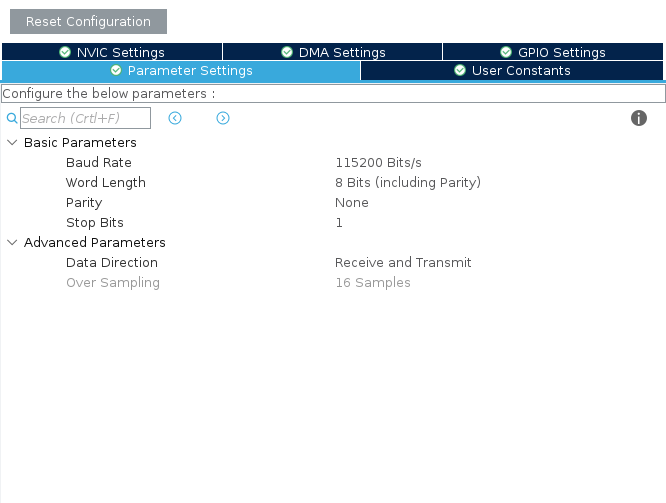
\includegraphics[width=\textwidth]{Pictures/parameter_uart.png}
        \caption{Baudrate,Format}
        \label{img: Parameter}
    \end{subfigure}
    %
    \begin{subfigure}{0.45\textwidth}
        \centering
        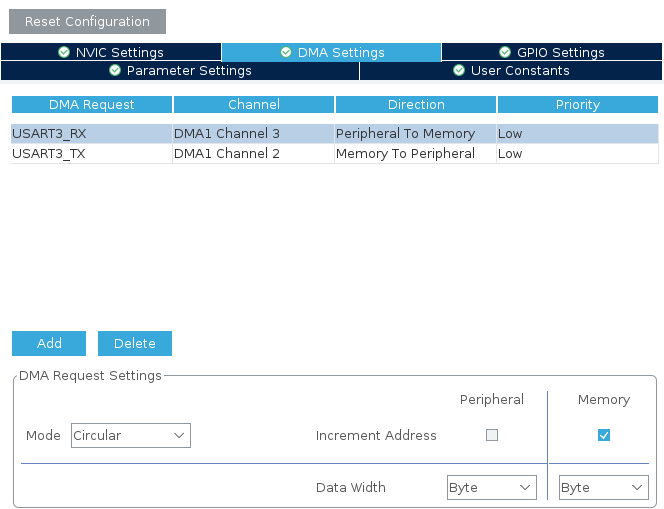
\includegraphics[width=\textwidth]{Pictures/dma_uart.png}
        \caption{DMA}
        \label{img: DMA}
    \end{subfigure}
    \caption{Konfiguration des \acp{UART}}
    \label{img: UART config}
  \end{figure}

  \subsubsection{STM32: Idle Line Detection}
  \label{subsub: Idle}

  Es ist von großem Vorteil, zu erkennen, wenn keine Daten mehr Empfangen werden, um das schreiben von sinnlosen Daten in den Buffer zu vermeiden.
  Deshalb wird eine s.g. \textit{Idle Line Detection} implementiert, welche erkennt, sobald keine Daten mehr empfangen werden.

  \newpage

  Der STM32 bietet dafür einen Interrupt, welcher manuell aktiviert werden muss \citep{STM32_Ref}. Um den Interrupt zu aktivieren, muss in der Datei
  \lstinline!stm32f1xx_it.c! die Funktion 
  
  \lstinline!void USARTX_IRQHandler(void)! folgendermaßen erweitert werden:

  \begin{lstlisting}
    if(__HAL_UART_GET_FLAG(&huartx,UART_FLAG_IDLE))
    {
        __HAL_UART_CLEAR_IDLEFLAG(&huartx);
        dma_info.timer = DMA_TIMEOUT_MS;
    }
  \end{lstlisting}

  Jedes mal, wenn ein Interrupt in Zusammenhang mit dem \ac{UART} ausgelöst wird, wird die Routine \lstinline!void USARTX_IRQHandler(void)! 
  aufgerufen  und geprüft, ob es sich um ein Idle Line Interrupt handelt \citep{STM32_Ref}. 

  \smallskip

  Es ist allerdings nicht ausreichend, nur zu prüfen, ob der Interrupt aufgetreten ist - es kann durchaus vorkommen, dass es sich nur um eine
  kurze Unterbrechung in der Kommunikation handelt. Deshalb wird die Funktionalität um einen Timeout erweitert. Wenn der Interrupt auftritt, wird
  gleichzeitig die Strukturvariable \lstinline!dma_info.timer! mit einer definierten Zeitwert \lstinline!DMA_TIMEOUT_MS! geladen.

  \smallskip

  Um für zukünftige Erweiterungen keinen Timer zu blockieren, wird für den Timeout der Systick-Timer (\ref{subsub: Timer}) genutzt. Dieser implementiert eine Routine,
  welche im 10ms-Takt aufgerufen wird. Diese Routine ist ebenfalls in der Datei \lstinline!stm32fxx_it.c! zu finden und wird um folgenden Code
  erweitert:

  \begin{lstlisting}
    if(dma_info.timer == 1)
    {
        dma_info.t_flag = 1;
        HAL_UART_RxCpltCallback(&huartx);
    }
    if(dma_info.timer) 
    { 
        --dma_info.timer; 
    }



  \end{lstlisting}
  
  Mittels dieser Erweiterung wird nun immer der Zähler des Timeouts dekrementiert, bis er eins erreicht. Wenn dies geschieht, wird ein Flag gesetzt
  und die Interruptroutine \lstinline!HAL\_UART\_RxCpltCallback(&huartx)! aufgerufen, in welcher anschließend der aufgetauchte Interrupt mittels des
  gesetzten Flags identifiziert und verarbeitet wird.
  
  \subsubsection{STM32: Empfangsinterrupt / DMA Circular Buffer}
  \label{subsub: Empfang}

  Während der Kommunikation mit \ac{UART} werden verschiedene Interrupts ausgelöst. Bei der Nutzung von \ac{DMA} werden Interrupts ausgelöst,
  wenn der Buffer halb oder ganz voll ist \citep{STM32_Ref}. Desweiteren wurde der \ac{uC} so konfiguriert, dass auch bei einem Idle Line Interrupt
  die entsprechende Interruptroutine aufgerufen wird \ref{subsub: Idle}.

  \smallskip

  Die Interruptroutine sind nach der Generation von Code mittels CubeMX in der Datei \lstinline!stm32f1xx_hal.c! als \lstinline!__weak!
  definiert, werden also neu gesetzt sobald sie ohne das Keyword \lstinline!__weak! definiert werden \citep{HAL_Description}. 

  \smallskip

  In \lstinline!main.c! wird die Interruptroutine mit dem Namen 
  \begin{lstlisting}
    void HAL_UART_RxCpltCallback(UART_HandleTypeDef *huart)
  \end{lstlisting}
  initialisiert. 
  
  \smallskip

  Die Variablen \lstinline!pos!, \lstinline!start! und \lstinline!length! werden für den Ringbuffer benötigt. Die Variable \lstinline!currCount! speichert die aktuelle Position des
  Ringbuffers und wird über den Befehl
  
  \begin{lstlisting}
    __HAL_DMA_GET_COUNTER(huart->hdmarx)
  \end{lstlisting}
  beschrieben.

  \smallskip

  Die Variable \lstinline!start! enthält die Startposition, ab welcher neue Daten im Ringbuffer enthalten sind. In der Variable \lstinline!length!
  ist die Länge der Daten gespeichert. Tritt ein Interrupt auf, weil der Empfangsbuffer voll ist, berechnet sich die Länge der empfangenen 
  Daten simpel durch folgenden Befehl:
  \begin{lstlisting}
    length = DMA_BUF_SIZE - start;
  \end{lstlisting}
  Es kann nun jedoch dazu kommen, dass nachdem der Buffer voll ist, ein Timeout-Interrupt ausgelöst wird. Um nun falsche Verarbeitung von 
  Daten zu verhindern, wird die aktuelle Position des Buffers auf die Größe des Buffers gesetzt.
  \begin{lstlisting}
    dma_info.prevCOUNT = DMA_BUF_SIZE;      
  \end{lstlisting}
  Wird nun ein Timeout-Interrupt ausgelöst, wird die Routine durch folgenden Code frühzeitig abgebrochen und das Flag rückgesetzt:
  \begin{lstlisting}
    if(dma_info.t_flag && currCOUNT == DMA_BUF_SIZE)
    {
        dma_info.t_flag = 0;
        return;
    }
  \end{lstlisting}